\section{Smart Grid -ready}

  Bundesverband Wärmepumpe e.V. (jäljenpänä BWP) on saksalainen lämpöpuppuyhdistys. BWP ylläpitää lämpöpumppujen ohjaukseen käytettävää rajapintaa määrittävää \gls{SG}-Ready-merkintää(\gls{SG} Ready label). \gls{SG}-Ready määrittelee pumpulle neljä eri toimintatilaa, joiden perusteella ulkoinen toimija kykenee ohjaamaan lämpöpumpun toimintaa. Toimintatilat yksi ja kaksi ovat yhteensopivia Saksassa käytetyn muunmuassa lämpöpumppuihin kohdistetutun energiantoimittajien suorittaman ohjauksen (EVU-Sperre\footnote{Energieversorgungsunternehmen}) kanssa. Ohjattava lämpöpumppu voidaan kytkeä energiatoimittajan toimesta pois päältä enimmillään kahdeksi tunniksi kerrallaan. Yhteen vuorokauteen taas voi sijoittua enintään kolme keskeytystä, jotka on pyritään sijoittamaan suurimman kulutuksen hetkiin. Kun kuluttajan tekee sähkösopimuksen, johon ohjaus kuuluu, saa hän vastavuoroisesti alennusta energian hinnasta.\parencite{SGReadyReg}

  SG-Readyn  kolmas ja neljäs toimintatila ovat sopivia ylituotannon kompensointiin niiden lisätessä lämpöpumppujen sähkönkulutusta. Eri toimintatilat on eritelty taulukossa \ref{sgready}.
  \begin{table}[h]
    \centering
    \caption[\gls{SG}-Ready toimintatilat]{\gls{SG}-Ready toimintatilat. Perustuu lähteeseen \parencite{SGReadyReg}.}
    \begin{tabular}{|c|c|p{3in}|}
      \hline
      \rowcolor{lightgray} toimintatila & looginen kytkentä & kuvaus \\\hline
      1 & 1 0 & Lämpöpumppu on kytkettynä pois päältä. Enintään kaksi tuntia kerrallaan enintään kolme kertaa vuorokaudessa \\\hline
      2 & 0 0 & Normaali toimintatila. Varaudutaan mahdolliseen kahden tunnin pysäytykseen. \\\hline
      3 & 0 1 & Suositeltu päälläolo. \\ \hline
      4 & 1 1 & Pakotettu päälläolo. Mahdollisesti myös lisävastuksen pakotettu päälläolo. \\\hline
    \end{tabular}
    \label{sgready}
  \end{table}
  Jokaiselle toimintatilalle on määritelty binäärinen arvo (0b00 -- 0b11), joka voidaan toteuttaa kahdella loogisella tilalla. SG-Ready ei ota kantaa siihen, miten nämä tilat tuodaan ohjattavalle laitteelle\marginpar{varmista}.\parencite{SGReadyReg}

  SG-Ready on korkean abstraktiotason rajapinta, joka tarjoaa keinoja ohjausrajapintojen yhtenäistämiseen. Alemman tason kommunikointi, johon siis SG-Ready ei ota kantaa, pitää määritellä ja toteuttaa toisella tasolla. Yksi alemman tason kommunikoinnissa yleisesti käytettävä standardi on Modbus-viestintäprotokolla.

\section{Modbus}

  Modbus on automaatiossa käytetty palvelin--asiakas-mallin viestintäprotokolla. Sen on alunperin kehittänyt vuonna 1979 yritys nimeltään Modicon käytettäväksi valmistamiens ohjelmoitavien logiikoiden eli \Gls{plc}:den väliseen viestintään. Nykyin Modicon on osa Ranskalaista Schneider Electriciä. Koska standardi on julkaistu avoimesti kaikkien käytettäväksi ja se on verrattain yksinkertainen, on se saavuttanut johtavan aseman teollisuudessa. Yleisimmille ohjelmointikielille on saatavilla modbus-standardin toteuttavat kirjastot, joiden avulla voidaan ohjelmallisesti  ohjata laitteita. Laajan levinneisyyden ansiosta modbus soveltuu monien eri valmistajien laitteiden järjestelmien kanssa käytettäväksi. Teollisuuden lisäksi protokollaa käytetään myös talo- ja kiinteistöautomaatiossa.\parencite{sousaPortugal, modbusAppSpec, modbusOrg}

  Vuonna 2004 Schneider Electric siirsi modbus-standardin hallinnan voittoa tavoittelemattomalle Modbus-järjestölle\footnote{Modbus Organization, Inc}. Järjestön muodostavat automaatiolaitteita valmistavat yritykset ja yksittäiset henkilöt ja sen tehtäviin kuuluu ylläpitää ja kehittää modbus-standardia ja siihen liittyviä documentteja sekä toimia etujärjestönä edistäen modbusin käyttöä. Modbusiin liittyvien documenttien ja julkaisujen avulla edistetään eri valmistajien järjestelmien välistä kommunikaatiota ja helpotetaan niiden integraatioita toisiinsa.  \parencite{modbusOrg}

  \subsection{viestintä ja tietomalli}

  Modbus-protokollan toiminta perustuu palvelinlaitteella sijaitsevien muistialueiden lukemiseen ja kirjoittamiseen kuvassa \ref{fig:c_s} kuvatun asiakas--palvelin-mallin (client--server model, ennen tunnettu termillä master-slave model) mukaan.  Lukemalla tietoja asiakaslaite kykenee seuraamaan palvelinlaitteen tilaa ja kirjoittamalla ohjaamaan sen toimintaa. Tietojen lukeminen ja kirjoittaminen tapahtuu protokollan määrittämien kysely, vastaus- ja virheviestien perusteella.\parencite{modbusAppSpec}

  \begin{figure}[h]
    \centering
    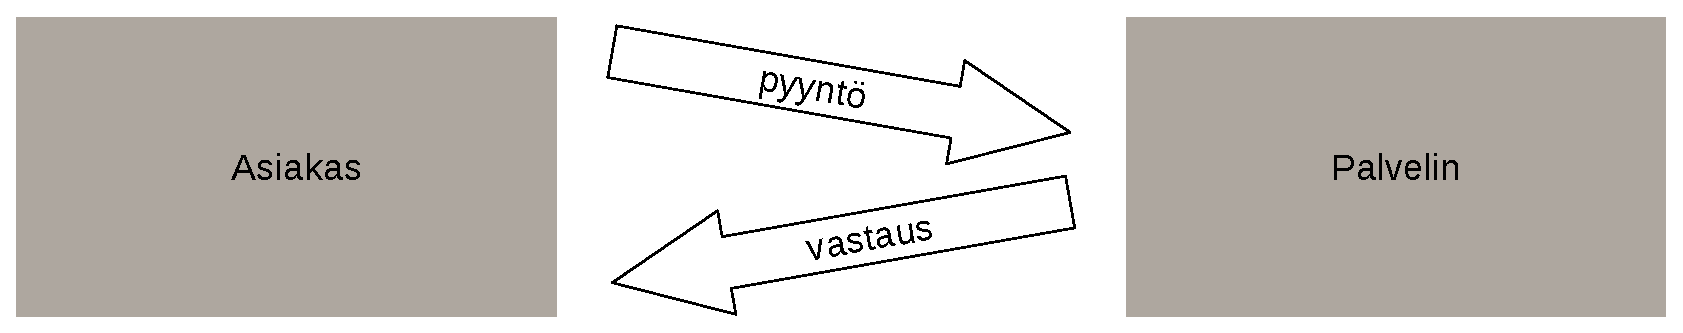
\includegraphics[width=1\textwidth]{figures/client_server}
    \caption[asiakas--palvelin-malli]{Asiakas--palvelin-malli.  Perustuen lähteeseen \parencite{modbusAppSpec}}
    \label{fig:c_s}
  \end{figure}

  Modbus-verkko muodostuu yhdestä asiakkaasta, ja yhdestä tai useammasta palvelimesta. Palvelimet yksilöidään kokonaislukuosoitteella väliltä 1--247, mikä rajoittaa samaan verkkoon kytkettyjen latteiden määrää.  Protokolla rajoittaa komminikointia niin, että kyselyitä lähettää vain asiakaslaite palvelinlaitteiden ainoastaan vastatessa niille osoitettuihin kyselyihin.\parencite{modbusSerialSpec} Tästä johtuen palvelinlaitteen eivät kykene itsenäisesti raportoimaan mahdollisesta virhetilanteesta tai tapahtumasta, vaan asiakaslaitteiden on jatkuvasti tehtävä kyselyitä pysyäkseen ajan tasalla. Tämä modbusin ominaisuus vähentää sen käyttökelpoisuutta, varsinkin, mikäli kommunikointiresurssit ovat rajalliset.

  Modbus-protokolla määrittelee lähetettäville kyselyille kaksi eri muotoa: täsmälähetys (unicast) ja monilähetys (multicast). Täsmälähetys osoitetaan tietylle palvelimelle ja vastaanotettuaan sen palvelin toimee sen mukaisesti. Monilähetys taas lähetetään osoitteella 0, jolloin kaikki palvelimet reagoivat kyselyyn.\parencite{modbusSerialSpec} Kerrallaan vain yksi laite verkossa voi toimia asiakkaana muiden toimiessa palvelimina. Tästä huolimatta yksittäinen laite voi kuitenkin toimia sekä palvelimena, että asiakkaana, kunhan tämä tapahtuu erillisissä verkoissa.\parencite{DincerRosen}

  Modbus-protokollan tietomalli koostuu palvelinlaitteella sijaitsevista muistialueista, jotka on jaettu taulukoihiin. Pääasialliset neljä muistialuetaulukkoa on kuvattu taulukossa \ref{taulukot}. Taulukoiden nimeäminen suomenkiellellä on haastavaa, joten se jätetään tekemättä.
  \begin{table}[h]
    \centering
    \caption[Modbus muistialuetaulukot.]{Modbus muistialuetaulukot. Perustuu lähteeseen \parencite{modbusAppSpec}.}
    \begin{tabular}{|l|l|l|}
      \hline
      \rowcolor{gray} taulukon tyyppi         & datatyyyppi      & asiakkaan oikeudet  \\ \hline
      \cellcolor{lightgray}Discretes Input    & 1 bitti          & vain luku           \\ \hline
      \cellcolor{lightgray}Coils              & 1 bitti          & luku/kirjoitus      \\ \hline
      \cellcolor{lightgray}Input Registers    & 16-bittinen sana & vain luku           \\ \hline
      \cellcolor{lightgray}Holding Registers  & 16-bittinen sana & luku/kirjoitus      \\ \hline
    \end{tabular}
    \label{taulukot}
  \end{table}
  1-bittisiä muistipaikkoja voidaan käyttää esimerkikksi päälläolotietojen välittämiseen, kun taas kahden tavun mittaisia muistipaikkoja voidaan käyttää esimerkiksi mitattujen arvojen ilmoittamiseen. Protokolla ei kuitenkaan määritä miten muistipaikkoja kuuluu käyttää, vaan tämä jätetään sovelluksen tekijän päätettäväksi. Kussakin taulukossa on 65536 erillistä osoitetta, joihin dataa voi tallentaa. Datan käsittely tapahtuu joko yksittäisen osoitteen perusteella tai sitten useampi perättäinen osoite kerrallaan.\parencite{modbusAppSpec}

  \subsection{Application data unit}

    Laitteissa toimivien sovellusten väliseen tiedonsiirtoon käytetään \gls{PDU}:a (Application Data Unit), joka koostuu funktiokoodista ja operaatioon tarvittavasta datasta. \gls{PDU}:ja on kolmenlaisia, ja ne on esitetty taulukossa \ref{pdu}.
    \begin{table}[h]
      \centering
      \caption[\gls{PDU}-tyypit.]{\gls{PDU}-tyypit. Perustuu lähteeseen \parencite{modbusAppSpec}.}
      \begin{tabular}{ccl}
        \cellcolor{green}Funktiokoodi (F)              & \cellcolor{green}Kyselyn data    & Kysely-PDU   \\
                                                       &                                  &              \\
        \cellcolor{green}Funktiokoodi (F)              & \cellcolor{green}Vastauksen data & Vastaus-PDU  \\
                                                       &                                  &              \\
        \cellcolor{red}Poikkeusfunktiokoodi (F + 0x80) & \cellcolor{red}Poikkeuskoodi     & Poikkeus-PDU \\
      \end{tabular}
      \label{pdu}
    \end{table}
    \gls{PDU}:n alun muodotaa funktiokoodi, joka on joko Modbus-protokollan tai käyttäjän määrittämä funktio. ADU:n loppuosa koostuu mahdollisesta datasta, jota palvelin tarvitsee suorittaakseen halutun toiminnon. Vastaus-PDU:un tulee sama funktiokoodi kuin kysely-PDU:un. Mikäli palvelin päätyy virhetilanteesee, joko virheellisen kysely-PDU:n tai sisäisen virheen takia, vastaa se asiakkaalle poikkeus-PDU:lla, joka muodostuu funktiokoodista, joka on yhdistettu heksakoodiin 0x80 ja poikkeuskoodista.\parencite{modbusAppSpec} Funktiokoodeista käytetyimmät liittyvät yksittäisten muistipaikkojen lukemiseen ja kirjoittamiseen\parencite{DincerRosen}. Lista yleisistä funktio- ja poikkeuskoodeista löytyy liitteestä \ref{app:modbus_funktio_koodit}.


  \subsection{protokollan rakenne}

    Modbus-protokollasta on totetutettu muutamia eri versioita:
    \begin{itemize}
      \item sarjaväyläversio eli Modbus Serial, joka muodostuu kahdesta muunnelmasta:
      \begin{itemize}
        \item Modbus \gls{RTU} ja
        \item Modbus ASCII,
      \end{itemize}
      \item Modbus TCP/IP ja
      \item Modbus Plus.
      \parencite{modbusAppSpec}
    \end{itemize}
    Edellisistä Modbus Plus on Schneider Electricin hallinnoima, eikä se ole avoimesti saatavilla. Modbus Plus on oma Modbusista eroava standardinsa, jota ei tässä käsitellä enempää.\parencite{seCom}

    Taulukossa \ref{rakenne} on Modbus-protokollaperhettä verrattu \gls{OSI}-malliin. Modbus-protokollan ylempi kerros, eli \gls{MBAP} sijoittuu \gls{OSI}-mallissa kerroseen 7, eli sovelluskerrokseen. \gls{MBAP}:n toimintaa on esitelty edellisessä kappaleissa. Sarjaväyläversiossa alempi kerros sijoittuu \gls{OSI}-mallissa kerrokseen 2 ja Modbus TCP/IP:n tapauksessa kerrokseen 5\footnote{\gls{OSI}-mallin teoreettisesta luonteesta johtuen tästä voinee esittää eroavia mielipiteitä.}.
    \begin{table}
      \centering
      \caption[Modbus-protokollan rakenne ja \gls{OSI}-malli]{Modbus-protokollan rakenne ja sen sovitus \gls{OSI}-malliin. Modbus-protokollaperhe sinisellä. Perustuu lähteisiin \parencite{osi, modbusSerialSpec, modbusTCPIPSpec}.}
      \begin{tabular}{|c|c|ccc}
        \cline{1-2}
        \multicolumn{2}{|c|}{OSI-mali}                                               & \multicolumn{3}{c}{}                                                                                                                                                                           \\ \hline
        \multicolumn{1}{|l|}{}                    &                                  & \multicolumn{3}{c|}{\cellcolor{yellow}SunSpec}                                                                                                                                                 \\ \cline{3-5}
        \multicolumn{1}{|l|}{7}                   & sovelluskerros                   & \multicolumn{3}{c|}{\cellcolor{blue}MBAP (Modbus-viestintäprotokolla)}                                                                                                                         \\ \hline
        6                                         & esityskerros                     &                                                         &                                                           & \multicolumn{1}{c|}{}                                                    \\ \cline{1-2} \cline{5-5}
        5                                         & istuntokerros                    &                                                         & \multicolumn{1}{c|}{}                                     & \multicolumn{1}{c|}{\cellcolor{blue}Modbus-\gls{TCP}}                    \\ \cline{1-2} \cline{5-5}
        4                                         & kuljetuskerros                   &                                                         & \multicolumn{1}{c|}{}                                     & \multicolumn{1}{c|}{\gls{TCP}}                                           \\ \cline{1-2} \cline{5-5}
        3                                         & verkkokerros                     &                                                         & \multicolumn{1}{c|}{}                                     & \multicolumn{1}{c|}{IP}                                                  \\ \hline
        2                                         & siirtokerros                     & \multicolumn{1}{c|}{\cellcolor{blue}Modbus-RTU}         & \multicolumn{1}{c|}{\cellcolor{blue}Modbus-ASCII}         & \multicolumn{1}{c|}{Ethernet, \dots}                                     \\ \hline
        1                                         & fyysinen kerros                  & \multicolumn{2}{c|}{RS-232 / RS-485}                                                                                & \multicolumn{1}{c|}{Ethernet, \dots}                                     \\ \hline
      \end{tabular}
      \label{rakenne}
    \end{table}

    \gls{MBAP} on kaikille Modbus-versioille yhteinen ja se mahdollistaa viestinnän laitteiden kesken erilaisten verkkojen ylitse. Välittettävät funktiokoodit ja data pakataa \gls{MBAP}:n toimesta PDU:ksi. Alemmassa keroksessa muodostetaan \gls{ADU}(application data unit), joka sisältää PDU:n lisäksi kohdelaitteen osoitteen ja tarkistussumman tai jos kyseessä on Modbus-TCP, \gls{MBAP}-otsikon. Erilaiset ADU:t on esitelty kuvassa \ref{fig:adu}.
    \begin{figure}[h]
      \centering
      
\includegraphics[width=1\textwidth]{figures/adu}
      \caption[ADU-tyypit]{Erilaiset ADU-tyypit.  Perustuen lähteisiin \parencite{modbusTCPIPSpec, modbusSerialSpec}}
      \label{fig:adu}
    \end{figure}

    Sarjaväylän yli toimivassa Modbusissa ADU siirretään käyttäen RS-485-standardia noudattavaa väylää tai RS-232-väylää pitkin. Oletuksena Modbus-standardi kehoittaa laitevalmistajia toteuttamaan ainakin RS-485-rajapinnan, RS-232-rajapinnan ollessa vapaaehtoinen. Modbus \gls{RTU} siirtää datan suoraan bitteinä. Modbus \gls{ASCII}:ssa taas jokainen tavu koodataan kahdeksi heksadesimaalimerkiksi ennen lähetystä, mikä heikentää sen tiedonsiirtokykyä. Modbus-standardi edellyttää, että kaikki laitteet tukevat ainakin Modbus RTU:ta Modbus ASCII:n ollessa suositeltu.\parencite{modbusSerialSpec}

    Modbus TCP/IP:tä käytettäessä Modbus-liikenne voi kulkea normaalin Internet-liikenteen mukana, mikä tekee siitä huomattavan joustavan ratkaisun. TCP-portti 502 on varattu Modbus-sovelluksille.\parencite{modbusTCPIPSpec} Koska ADU:t lähetetään TCP-kehyksessä, niihin ei tarvitse laskea eikä lisätä tarkistussummaa. TCP-protokolla huolehtii paketin (kehys + ADU) perille pääsystä ja mahdollisista uudelleenlähetyksistä. Tietosuojasta voidaan huolehtia käyttämällä kommunikointiin \gls{VPN}-yhteyttä. Toinen turvallisuutta parantava keino on käyttää komminikointiin MODBUS/TCP Security -standardin mukaista TLS-salausta, jolloin liikenne kohdistetaan TCP-porttiin 802\parencite{modbusTCPIPTLSSpec}.
